O ADC (\emph{Analog-To-Digital Converter}) é um periférico responsável por realizar a conversão de uma grandeza analógica de tensão para um valor correspondente digital. Para realizar esta conversão pode-se implementar vários  tipos circuito, como o conversor flash, ou o conversor de aproximações sucessivas, ou ainda conversor integrador simples ou de rampa dupla. Porém o  circuito de conversão mais usado em circuito integrados atualmente é o conversor de aproximações sucessivas, o qual também usado como AD no Tiva TM4C1294NCPDT. 


\section{ADC de Aproximações Sucessivas}

\begin{figure}[H]
	\centering
	\fbox{
	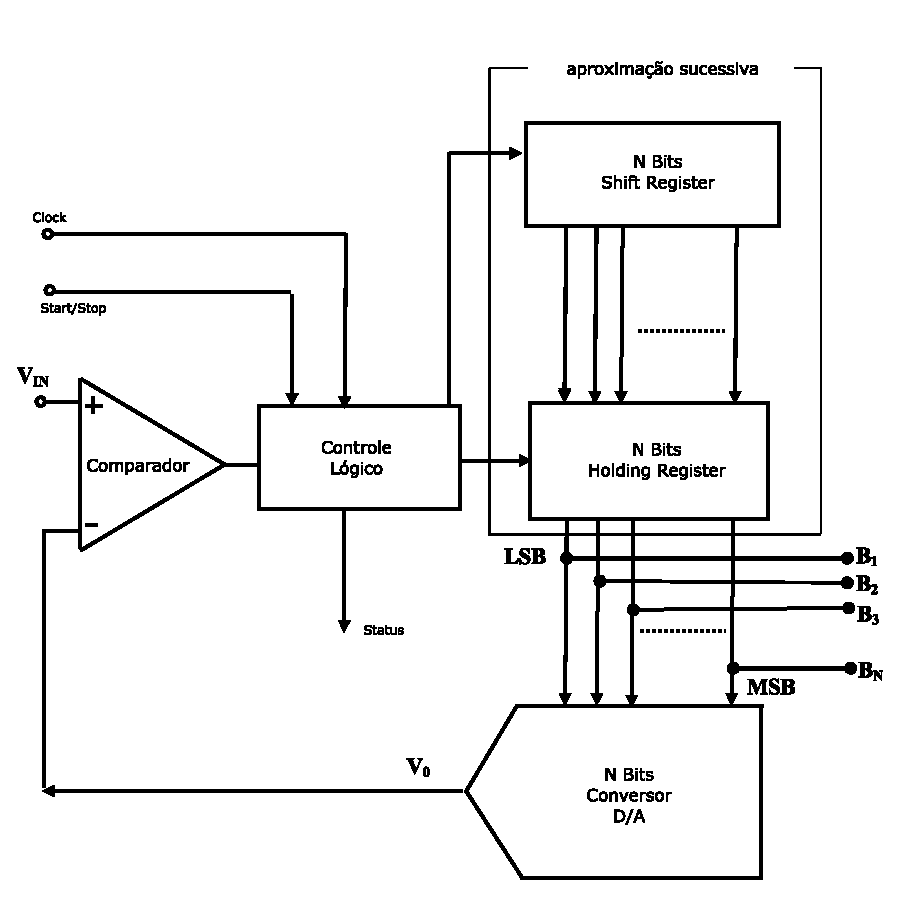
\includegraphics[width=0.85\textwidth] {figuras/ConversorAD.eps}}
	\caption{Conversor A/D tipo Aproximação Sucessiva}
	\label{fig:ConversorAD}
\end{figure}

 A figura \ref{fig:ConversorAD} apresenta o diagrama básico de funcionamento de um conversor de aproximações sucessivas. Nota-se que tal conversor utiliza a técnica de realimentação para relacionar uma voltagem analógica de entrada com um código digital, através de um conversor DA (\emph{Digital-To-Analog Converter}) e um comparador. O processo de conversão inicia quando o \emph{Shift Register} e o \emph{Holding Register} são zerados, e então o MSB (\emph{Most Significant Bit}) do \emph{Holding Register} vai para nível alto. Em seguida o comparador relaciona a saída do conversor DA com a tensão $V_{IN}$. Se $V_{O} < V_{IN}$ a conversão chega ao fim, porém se isso não for verdade a etapa se repete e MSB vai para nível baixo e o segundo SB vai para nível alto. E assim se dá a conversão. 

\section{ADC do TM4C1294NCPDT}

O Tiva TM4C1294NCPDT possui 2 módulos de conversão AD  de 12-bit, que podem ser usados em qualquer um das 20 entradas de sinal analógico. É possível realizar amostragens sequenciais entre os canais ou no mesmo canal repetidamente com intervalos de tempo  programáveis. Cada módulo AD possui 8 comparadores que possibilitam realizar comparações entre os sinais de entrada e  valores pré-definidos, para que assim possa ser realizado as mais diversas operações.  Ainda é possível usar um \emph{trigger} diferente para cada um dos módulos, ou usar um \emph{trigger} para acionar ambos os módulos.

A tabela \ref{tab:CanaisADC} apresenta os pinos de entrada para os módulos ADC0 e ADC1, com a descrição do nome do pino de entrada, o numero referente a este pino, sua função e o tipo de \emph{buffer} usado. Nesta mesma tabela temos o  pino chamado de $VREFA+$ que é o pino da tensão de referência usado pelo AD. O $VREFA+$ corresponde o valor máximo que o conversor DA, usado pelo AD para realizar a comparação com a tensão de entrada, pode atingir. 

A tensão $VREFA+$ é extremamente importante para se realizar a conversão AD, pois se este valor não for selecionado de forma adequada pode-se acarretar problemas no valor digital. A tensão $VREFA+$ pode ser alternada entre uma fonte de referência interna ou externa. 

\begin{center}
\begin{longtable}{|c|c|c|c|c|c|}
	\rowcolor[HTML]{000000}
	{\color[HTML]{FFFFFF} Pino} & {\color[HTML]{FFFFFF} $n^{o}$} & {\color[HTML]{FFFFFF} Mux/Função} & {\color[HTML]{FFFFFF} Tipo} & {\color[HTML]{FFFFFF} Buffer} & {\color[HTML]{FFFFFF} Descrição}            \\
	AIN0                        & 12                             & PE3                               & I                           & Analógico                     & ADC - Entrada 0                             \\
	\hline
	AIN1                        & 13                             & PE2                               & I                           & Analógico                     & ADC - Entrada 1                             \\
	\hline
	AIN2                        & 14                             & PE1                               & I                           & Analógico                     & ADC - Entrada 2                             \\
	\hline
	AIN3                        & 15                             & PE0                               & I                           & Analógico                     & ADC - Entrada 3                             \\
	\hline
	AIN4                        & 128                            & PD7                               & I                           & Analógico                     & ADC - Entrada 4                             \\
	\hline
	AIN5                        & 127                            & PD6                               & I                           & Analógico                     & ADC - Entrada 5                             \\
	\hline
	AIN6                        & 126                            & PD5                               & I                           & Analógico                     & ADC - Entrada 6                             \\
	\hline
	AIN7                        & 125                            & PD4                               & I                           & Analógico                     & ADC - Entrada 7                             \\
	\hline
	AIN8                        & 124                            & PE5                               & I                           & Analógico                     & ADC - Entrada 8                             \\
	\hline
	AIN9                        & 123                            & PE4                               & I                           & Analógico                     & ADC - Entrada 9                             \\
	\hline
	AIN10                       & 121                            & PB4                               & I                           & Analógico                     & ADC - Entrada 10                            \\
	\hline
	AIN11                       & 120                            & PB5                               & I                           & Analógico                     & ADC - Entrada 11                            \\
	\hline
	AIN12                       & 4                              & PD3                               & I                           & Analógico                     & ADC - Entrada 12                            \\
	\hline
	AIN13                       & 3                              & PD2                               & I                           & Analógico                     & ADC - Entrada 13                            \\
	\hline
	AIN14                       & 2                              & PD1                               & I                           & Analógico                     & ADC - Entrada 14                            \\
	\hline
	AIN15                       & 1                              & PD0                               & I                           & Analógico                     & ADC - Entrada 15                            \\
	\hline
	AIN16                       & 18                             & PK0                               & I                           & Analógico                     & ADC - Entrada 16                            \\
	\hline
	AIN17                       & 19                             & PK1                               & I                           & Analógico                     & ADC - Entrada 17                            \\
	\hline
	AIN18                       & 20                             & PK2                               & I                           & Analógico                     & ADC - Entrada 18                            \\
	\hline
	AIN19                       & 21                             & PK3                               & I                           & Analógico                     & ADC - Entrada 19                            \\
	\hline
	&                                &                                   &                             &                               & A tensão de referência                      \\
	&                                &                                   &                             &                               & \multicolumn{1}{l|}{é usada pelo AD para}    \\
	&                                &                                   &                             &                               & \multicolumn{1}{l|}{fixar o valor máximo de} \\
	\multirow{-4}{*}{VREFA+}    & \multirow{-4}{*}{9}            & \multirow{-4}{*}{fixo}            & \multirow{-4}{*}{-}         & \multirow{-4}{*}{Analógico}   & \multicolumn{1}{l|}{conversão.}  \\ 
	\hline
	\caption{Canais de Entrada ADC - Tiva TM4C1294NCPDT \cite{DATASHEET_TIVA} }
	\label{tab:CanaisADC}
\end{longtable}
\end{center}

\section{Na TivaWare}

As principais funções, da biblioteca TivaWare, responsáveis pela configuração e utilização do ADC, são listadas a seguir.

\begin{lstlisting}[style=funcao]
	void ADCSequenceConfigure(uint32_t ui32Base,
							  uint32_t ui32SequenceNum,
							  uint32_t ui32Trigger,
							  uint32_t ui32Priority)
\end{lstlisting}

Configurações básicas do ADC especificado.

\begin{description}
	\item [\ttbu{ui32Base}]\hfill \\
	Base do ADC a ser configurado. Normalmente \textbf{ADC\emph{k}\_BASE}, onde \textbf{\emph{k}} é a letra identificadora do periférico.
	
	\item [\ttbu{ui32SequenceNum}]\hfill \\
	Número da sequência de amostragem.
	
	\item [\ttbu{ui32Trigger}]\hfill \\
	Evento que aciona o amostrador. Definido no formato \textbf{ADC\_TRIGGER\_\emph{k}}, onde \textbf{\emph{k}} pode assumir um dos valores:
	\begin{itemize}
		\item \textbf{PROCESSOR} amostragem iniciada por comando de software.
		\item \textbf{COMP0} amostragem iniciada pelo comparador 0 do ADC.
		\item \textbf{COMP1} amostragem iniciada pelo comparador 1 do ADC.
		\item \textbf{COMP2} amostragem iniciada pelo comparador 2 do ADC.
		\item \textbf{EXTERNAL} amostragem iniciada por uma GPIO de entrada configurada.
		\item \textbf{TIMER} amostragem iniciada pelo temporizador.
		\item \textbf{PWM0} amostragem iniciada pelo PWM 0.
		\item \textbf{PWM1} amostragem iniciada pelo PWM 1.
		\item \textbf{PWM2} amostragem iniciada pelo PWM 2.
		\item \textbf{PWM3} amostragem iniciada pelo PWM 3.
		\item \textbf{ALWAYS} amostragem iniciada repetida e continuamente
	\end{itemize}
\end{description}

\begin{lstlisting}[style=funcao]
	void ADCSequenceStepConfigure(uint32_t ui32Base,
								  uint32_t ui32SequenceNum,
								  uint32_t ui32Step,
								  uint32_t ui32Config)
\end{lstlisting}

Configura o intervalo de amostragem do ADC especificado.

\begin{description}
	\item [\ttbu{ui32Base}]\hfill \\
	Base do ADC a ser configurado. Normalmente \textbf{ADC\emph{k}\_BASE}, onde \textbf{\emph{k}} é a letra identificadora do periférico.
	
	\item [\ttbu{ui32SequenceNum}]\hfill \\
	Número da sequência de amostragem.
	
	\item [\ttbu{ui32Step}]\hfill \\
	Intervalo de amostragem do ADC.
	
	\item [\ttbu{ui32Config}]\hfill \\
	Configuração da amostragem. Pacote de OU lógico de valores no formato \textbf{ADC\_CTL\_\emph{k}}, onde \textbf{\emph{k}} pode assumir os valores:
	\begin{itemize}
		\item \textbf{TS} amostragem do sensor de temperatura interno.
		\item \textbf{IE} amostragem gera interrupção.
		\item \textbf{END} amostragem por sequencia e seleção.
		\item \textbf{D} amostragem por seleção diferencial.
		\item \textbf{CH\emph{k}} seleciona canal de entrada como canal \textbf{\emph{k}}, onde \textbf{\emph{k}} assume valores de 0 a 23.
		\item \textbf{CMP\emph{k}} seleciona comparador \textbf{\emph{k}} para ser utilizado, onde \textbf{\emph{k}} assume valores de 0 a 7.
	\end{itemize}
\end{description}

\begin{lstlisting}[style=funcao]
	void ADCSequenceEnable(uint32_t ui32Base,
						   uint32_t ui32SequenceNum)
\end{lstlisting}

Habilita a sequência de amostragem.

\begin{description}
	\item [\ttbu{ui32Base}]\hfill \\
	Base do ADC a ser configurado. Normalmente \textbf{ADC\emph{k}\_BASE}, onde \textbf{\emph{k}} é a letra identificadora do periférico.
	
	\item [\ttbu{ui32SequenceNum}]\hfill \\
	Número da sequência de amostragem.
\end{description}

\begin{lstlisting}[style=funcao]
	void ADCSequenceDisable(uint32_t ui32Base,
							uint32_t ui32SequenceNum)
\end{lstlisting}

Desabilita a sequência de amostragem.

\begin{description}
	\item [\ttbu{ui32Base}]\hfill \\
	Base do ADC a ser configurado. Normalmente \textbf{ADC\emph{k}\_BASE}, onde \textbf{\emph{k}} é a letra identificadora do periférico.
	
	\item [\ttbu{ui32SequenceNum}]\hfill \\
	Número da sequência de amostragem.
\end{description}

\begin{lstlisting}[style=funcao]
	int32_t ADCSequenceDataGet(uint32_t ui32Base,
							   uint32_t ui32SequenceNum,
							   uint32_t *pui32Buffer)
\end{lstlisting}

Pega o valor gerado na amostragem.

\begin{description}
	\item [\ttbu{ui32Base}]\hfill \\
	Base do ADC a ser lido. Normalmente \textbf{ADC\emph{k}\_BASE}, onde \textbf{\emph{k}} é a letra identificadora do periférico.
	
	\item [\ttbu{ui32SequenceNum}]\hfill \\
	Número da sequência de amostragem.
	
	\item [\ttbu{pui32Buffer}]\hfill \\
	Ponteiro para uma região de memória alocada. Onde será armazenado o valor lido.
\end{description}

\begin{lstlisting}[style=funcao]
	int32_t ADCSequenceDataGet(uint32_t ui32Base,
							   uint32_t ui32SequenceNum,
							   uint32_t *pui32Buffer)
\end{lstlisting}

Pega o valor gerado na amostragem.

\begin{description}
	\item [\ttbu{ui32Base}]\hfill \\
	Base do ADC a ser lido. Normalmente \textbf{ADC\emph{k}\_BASE}, onde \textbf{\emph{k}} é a letra identificadora do periférico.
	
	\item [\ttbu{ui32SequenceNum}]\hfill \\
	Número da sequência de amostragem.
	
	\item [\ttbu{pui32Buffer}]\hfill \\
	Ponteiro para uma região de memória alocada. Onde será armazenado o valor lido.
\end{description}

\begin{lstlisting}[style=funcao]
	int32_t ADCSequenceOverflow(uint32_t ui32Base,
								uint32_t ui32SequenceNum)
\end{lstlisting}

Informa se houve uma perda de leitura, antes de ter lido o valor antigo ocorreu uma nova amostragem.

\begin{description}
	\item [\ttbu{ui32Base}]\hfill \\
	Base do ADC a ser lido. Normalmente \textbf{ADC\emph{k}\_BASE}, onde \textbf{\emph{k}} é a letra identificadora do periférico.
	
	\item [\ttbu{ui32SequenceNum}]\hfill \\
	Número da sequência de amostragem.
\end{description}

\begin{lstlisting}[style=funcao]
	void ADCProcessorTrigger(uint32_t ui32Base,
							 uint32_t ui32SequenceNum)
\end{lstlisting}

Causa uma leitura do ADC invocada pelo processador. Gatilho por software.

\begin{description}
	\item [\ttbu{ui32Base}]\hfill \\
	Base do ADC a ser chamado. Normalmente \textbf{ADC\emph{k}\_BASE}, onde \textbf{\emph{k}} é a letra identificadora do periférico.
	
	\item [\ttbu{ui32SequenceNum}]\hfill \\
	Número da sequência de amostragem.
\end{description}

\begin{lstlisting}[style=funcao]
	void ADCIntRegister(uint32_t ui32Base,
						uint32_t ui32SequenceNum,
						void (*pfnHandler)(void))
\end{lstlisting}

Configura rotina de tratamento de interrupção do ADC.

\begin{description}
	\item [\ttbu{ui32Base}]\hfill \\
	Base do ADC a ser configurada. Normalmente \textbf{ADC\emph{k}\_BASE}, onde \textbf{\emph{k}} é a letra identificadora do periférico.
	
	\item [\ttbu{ui32SequenceNum}]\hfill \\
	Número da sequência de amostragem.
	
	\item [\ttbu{pfnIntHandler}]\hfill \\
	Ponteiro da função de tratamento. Esta não deve receber nada como parâmetro e nem retornar nada.
	
\end{description}

\begin{lstlisting}[style=funcao]
	void ADCIntEnable(uint32_t ui32Base,
					  uint32_t ui32SequenceNum)
\end{lstlisting}

Habilita as interrupções do ADC.

\begin{description}
	\item [\ttbu{ui32Base}]\hfill \\
	Base do ADC a ser configurada. Normalmente \textbf{ADC\emph{k}\_BASE}, onde \textbf{\emph{k}} é a letra identificadora do periférico.
	
	\item [\ttbu{ui32SequenceNum}]\hfill \\
	Número da sequência de amostragem.
\end{description}

\begin{lstlisting}[style=funcao]
	void ADCIntDisable(uint32_t ui32Base,
					   uint32_t ui32SequenceNum)
\end{lstlisting}

Habilita as interrupções do ADC.

\begin{description}
	\item [\ttbu{ui32Base}]\hfill \\
	Base do ADC a ser configurada. Normalmente \textbf{ADC\emph{k}\_BASE}, onde \textbf{\emph{k}} é a letra identificadora do periférico.
	
	\item [\ttbu{ui32SequenceNum}]\hfill \\
	Número da sequência de amostragem.
\end{description}

\begin{lstlisting}[style=funcao]
	void ADCIntClear(uint32_t ui32Base,
					 uint32_t ui32SequenceNum)
\end{lstlisting}

Limpa a \emph{flag} de interrupções do ADC.

\begin{description}
	\item [\ttbu{ui32Base}]\hfill \\
	Base do ADC a ser configurada. Normalmente \textbf{ADC\emph{k}\_BASE}, onde \textbf{\emph{k}} é a letra identificadora do periférico.
	
	\item [\ttbu{ui32SequenceNum}]\hfill \\
	Número da sequência de amostragem.
\end{description}

\section{Exemplo}

A seguir, é apresentado um código de configuração do ADC. Um exemplo mais elaborado é apresentado na Seção \ref{sec:exPwm}.

\begin{lstlisting}[style=citacao]
// Habilita ADC0
MAP_SysCtlPeripheralEnable(SYSCTL_PERIPH_ADC0);
// Aguarda 3 SysCtlDelay. Aproximadamente 10 ciclos de clock
MAP_SysCtlDelay(3);

// Desabilitar Interrupcao do ADC para configura-la
MAP_IntDisable(INT_ADC0SS0);
MAP_ADCIntDisable(ADC0_BASE, 0);
MAP_ADCSequenceDisable(ADC0_BASE, 0);

//Configurando ADC
MAP_ADCHardwareOversampleConfigure(ADC0_BASE, 4);
MAP_ADCSequenceConfigure(ADC0_BASE, 0,
	ADC_TRIGGER_PROCESSOR, 0);
MAP_ADCSequenceStepConfigure(ADC0_BASE, 0, 0,
	ADC_CTL_IE | ADC_CTL_END | ADC_CTL_CH0);
MAP_ADCSequenceEnable(ADC0_BASE, 0);

// Habilitando Interrupcao do ADC
MAP_ADCIntClear(ADC0_BASE, 0);
MAP_ADCIntEnable(ADC0_BASE, 0);
MAP_IntEnable(INT_ADC0SS0);
\end{lstlisting}
